\thispagestyle{plain}
\begin{titlepage}

\begin{center}

\vspace*{10ex}
\huge{\textbf{\titel}}\\[4ex]
%\Large{\untertitel}\\[8ex]
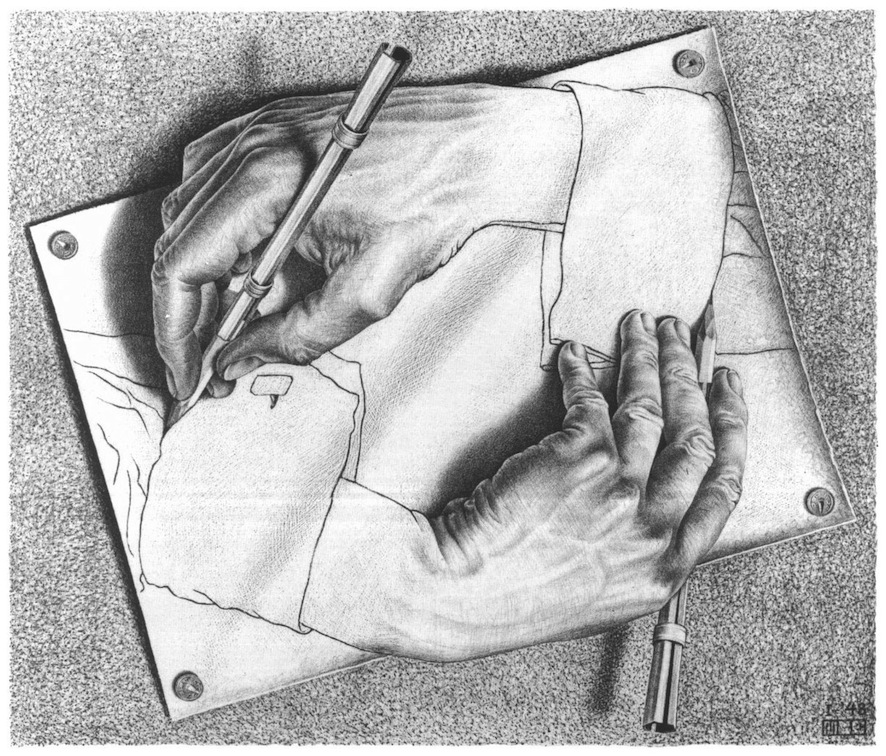
\includegraphics[width=150mm]{cover_escher.jpg}

\thispagestyle{empty}
\cleardoublepage
	
\vspace*{12ex}

\huge{\textbf{\titel}}\\[5ex]
%\Large{\untertitel}\\[10ex]

\large{\textit{\art}}\\
\large{\textit{\fachgebiet}}\\[14ex]

\normalsize
\begin{tabular}{w{5.4cm}p{6cm}}
 penned by: & \quad \autor\\
 mail address: & \quad \mail\\
 matriculation nr.: & \quad \matrikelnummer\\
 area of studies: & \quad \studienbereichA \\
 			& \quad \studienbereichB \\[2ex]
 censor: & \quad \gutachter\\
 second censor: & \quad \zweitgutachter\\
 supervisor: & \quad \betreuer\\[2ex]
 filing date: & \quad \abgabe
\end{tabular}

\tiny \noindent \\[12ex]
\copyright 2012 by \textit{Lukas N.P. Egger}, all Rights Reserved. The cover was created by \textit{Sivan Lutaty}, inspired by the work of \textit{M.C. Escher}.\\
This work is licensed under a Creative Commons Attribution-NonCommercial 3.0 Unported (\href{http://creativecommons.org/licenses/by-nc/3.0/}{CC BY-NC 3.0}).
\begin{figure}[hb]
\centering

\includegraphics[scale=0.75]{creative_commons.png}
\end{figure}








\end{center}
\end{titlepage}
